\documentclass[12pt,a4paper]{article}
\usepackage[pdftex]{graphicx}
\graphicspath{{Image/}}
\usepackage{epstopdf}
\usepackage{float}
\usepackage{amsmath}
\usepackage{mathtools}
\DeclarePairedDelimiter\abs{\lvert}{\rvert}
\DeclarePairedDelimiter\norm{\lVert}{\rVert}
\usepackage{esint}
\usepackage{amsfonts}
\usepackage{times}
\usepackage[top=.6 in, left=0.9in, right=0.9in]{geometry}
\usepackage{bbm}
\usepackage{dsfont}
\usepackage{enumerate}
\usepackage{titlesec}
\newcommand{\rn}{\mathbb{R}}
\newcommand{\E}{\mathbb{E}}
\newcommand{\Gn}{\mathbb{G}_{n}}
\newcommand{\G}{\mathbb{G}}
\newcommand {\tab}{\hspace{10 mm}}
\DeclareMathOperator*{\argmax}{arg\,max}
\DeclareMathOperator*{\argmin}{arg\,min}
\titleformat{\section}[block]{\large \it \filcenter}{}{0.5 ex}{}
\titleformat{\subsection}[block]{\small\it \filcenter}{}{0.5 em}{}
\titleformat{\subsubsection}[block]{\small\it \filcenter}{}{0.5 em}{}
\title{Empirical Methods in Economics\\\small{Assignment II}}
\date{Orville D. Mondal\\ $26^{th}$ of September, 2018\vspace{-3ex}}
\begin{document}
\maketitle
\begin{enumerate}
\item The demand for either product is around 0.4223, when the price of either equals 1, and valuations are both 2.
\item The starting value for this problem was $(P_{A},P_{B})=(1,4)$. The process converged in 9 iterations, taking 0.010425 seconds to do so. The equilibrium prices are 1.598942 for either commodity, which is reasonable, given the symmetric nature of the marginal cost and marginal revenue, along with the fact that valuations for both agents are the same.\par As to how one actually solves this problem: we need to find a solution to the following system of equations:
    \[\frac{1+\exp(v_{A}-P_{A})+\exp(v_{B}-P_{B})}{1+\exp(v_{j}-P_{j})}-P_{i}=0,\text{ for $i\neq j$, $i=A,B$.}\]
\item Gaus-Seidel is, in fact, faster. It converges in 0.0057 seconds, i.e. it is almost twice as fast. However, it takes \emph{many} more iterations: 48, compared to 9.\par Why Gauss-Seidel results in faster convergence is not very clear to me. In the language of game theory, and Cournot, in particular, though, the method mirrors the process of \emph{rationalisation}. A \emph{rationalisable} strategy is precisely one that survives the sort of iteration which Gauss-Seidel employs\footnote{This observation is due to Joonkyo Hong}.
\item This updating rule also leads to convergence. In fact, it takes fewer iterations than Gauss-Sidel (18, in this case, versus 48), although it takes slightly longer (0.0063 versus 0.0057 seconds). It is faster than Broyden (0.01 seconds).
\item As one would expect, equilibrium price paid is rising in one's value for a product, while falling in the valuation for an alternative product. Equal valuations lead to equal equilibrium prices. The figure is on the next page.\newpage
\begin{figure}
\centering
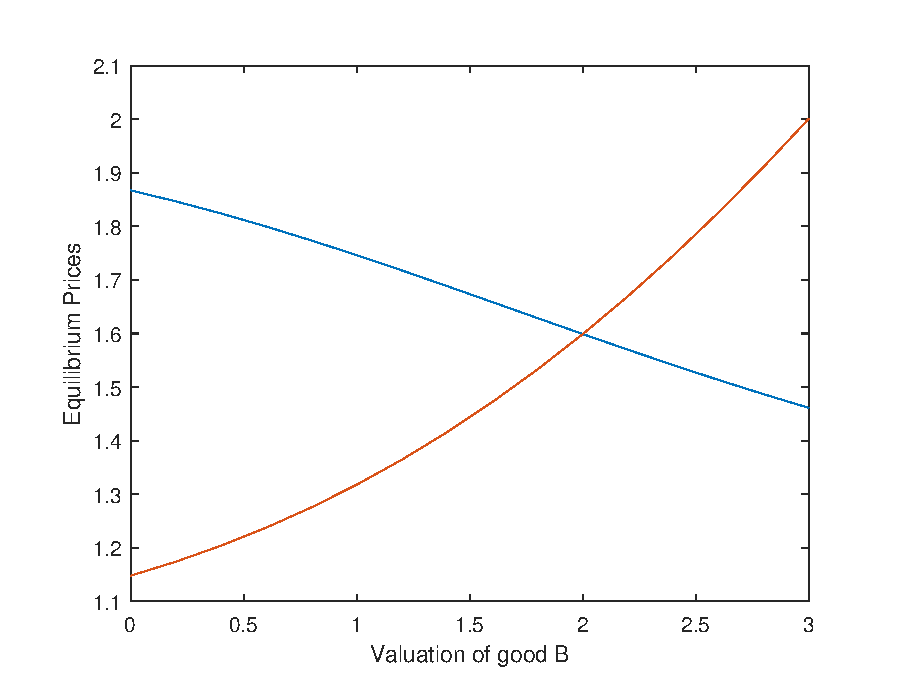
\includegraphics[width=0.8\textwidth]{fig1.eps}
\caption{Change in prices, responding to changes in valuation of B. The red line represents $P_{B}$, while the blue line represents $P_{A}.$}
\end{figure}
\end{enumerate}
\end{document} 